\chapter{History}


\section{Henri Poincare}
(Source: Wikipedia)

Poincar\'{e} was born on 29 April 1854 in City Ducale neighborhood, Nancy into an influential family.
\begin{figure}[hbt!]
\centering
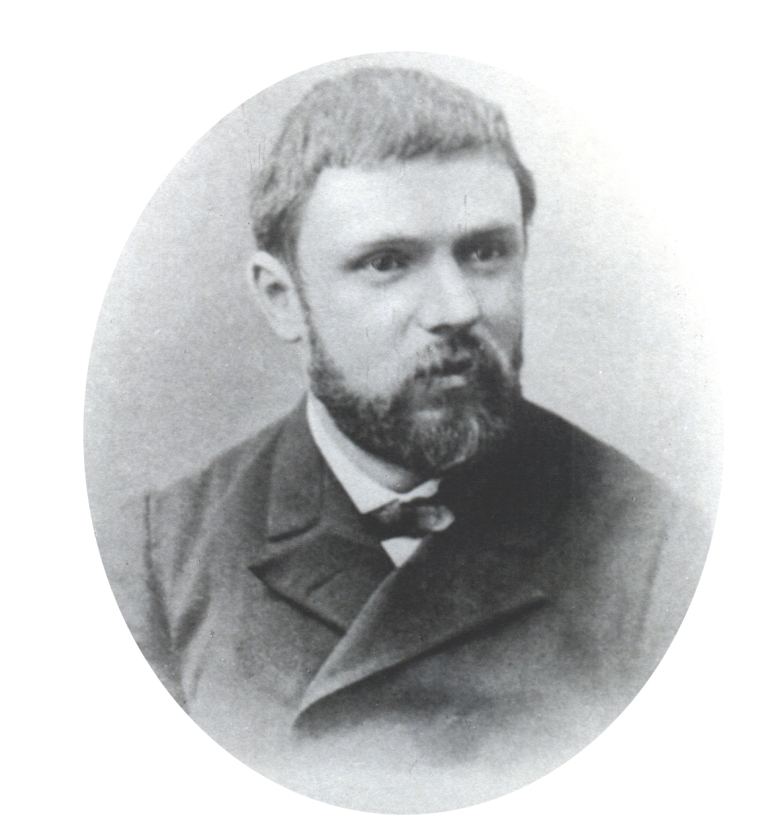
\includegraphics[width=.5\textwidth]{./images/poincare1.jpg}
\caption{Henri Poincare}\label{fig1}
\end{figure}


His father Leon Poincar\'{e} (1828-1892) was a professor of medicine at the University of Nancy. His younger sister Aline married the spiritual philosopher Emile Boutroux. Another notable member of Jules' family was his cousin, Raymond Poincar\'{e}, who would become the President of France, 1913 to 1920, and a fellow member of the Acad\'{e}mie francaise. He was raised in the Roman Catholic faith. However, he rejected Christianity in later life and became an atheist.

Henri was a precocious student who rose immediately to the top of his class, excelling in both science and letters. At age 13, his teacher told his mother that “Henri will become a mathematician... I would say a great mathematician” (Bellivier 1956: 78). During the Franco-Prussian war in 1870 the Germans occupied Nancy and the Poincar\'{e} family was obliged to billet the secretary of the civil commissar of Nancy, with whom Henri would have a round of conversation each night after dinner in order to improve his German.

In 1871, Poincar\'{e} passed the exams in letters with the grade "good" and that in science with the grade "fair". He received a zero in mathematics for answering a different question from the one that was asked, apparently having misunderstood the question. He then took the preparatory classes in mathematics and was first in his class, also first in the academic competition and first in the national competition (concours g\'{e}n\'{e}ral) in elementary mathematics. In Paris, he entered the École Polytechnique in 1873 and after graduating in 1875 (second in his class having apparently lost points for his inability to draw), entered the \'{E}cole des Mines. After brief service as a mine inspector, he submitted a dissertation on partial differential equations and he was then put in charge of the course on differential and integral calculus at the University of Caen.

In 1880, he submitted a memoir resolving a problem in the theory of differential equations to the competition for the grand prize in mathematics of the Academy of Sciences in Paris. Here for the first time he made use of non-Euclidean geometry, which was seen by most of his contemporaries as purely speculative. Poincar\'{e} married Louise Poulain d'Andecy on April 20, 1881 and was soon thereafter put on the faculty of sciences at the University of Paris. In 1886 he succeeded G. Lippmann in the chair of mathematical physics and probability. In 1896 he took the chair of mathematical astronomy and celestial mechanics, in 1902 he was named professor of theoretical electricity at the school of the post and telegraph and in 1904 professor of general astronomy at the \'{E}cole Polytechnique. Poincar\'{e} also worked at the French Bureau des Longitudes from 1893 (Galison 2003).

In 1889, Poincar\'{e} won the prize from the King of Sweden for a question posed by Weierstrass on the stability of the solar system, that is to say, the three-body (or n-body) problem in classical mechanics. Despite a mathematical error which he discovered at the last moment (after questions raised by the Swedish mathematician Lars Edvard Phragm\'{e}n) and frantically corrected, the work was important for its use of topology and as a founding document in chaos theory, for Poincar\'{e} showed that in general, the stability of such systems cannot be demonstrated. It is also in this context that he proved his famous recurrence theorem.

Poincar\'{e} joined the French Academy of Sciences in 1887 and became its president in 1906. On the basis of his three books on philosophical and general problems in science, he was elected to the Académie Française in 1908. He also became a corresponding member of many international scientific organizations. Poincar\'{e}'s extensive correspondence demonstrates the extent of his relations with the scientific community of his time (Nabonnand 1999; Walter 2007). His travel included a trip to America to give a lecture at the St. Louis World's Fair in 1904. He also co-signed a report that played an important role in the rehabilitation of Dreyfus.


\begin{figure}[hbt!]
\centering
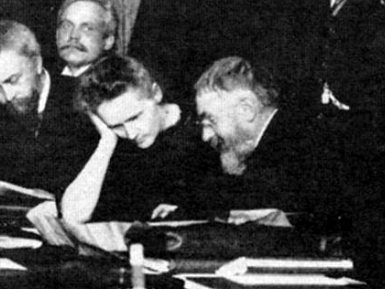
\includegraphics[width=.5\textwidth]{./images/solvay.jpg}
\caption{Henri Poincare with Marie Curie on the 1911 Solvay conference}\label{fig1}
\end{figure}

Poincar\'{e} is also famous for his 1904 conjecture concerning the topology of three-dimensional spheres, which remained one of the major unsolved problems in mathematicsuntil very recently, the Russian mathematician Grigori Perelman succeeded in demonstrating it nearly one hundred years later. Poincaré lectured on contemporary mathematical physics for years and was very much abreast of current developments. In all he published over five hundred scientific papers and over thirty books. He died from an embolism, at age fifty eight, on 17 July 1912, and was buried inside the Poincare family vault in the cemetery of Montparnasse, Paris.
\clearpage

